\chapter{Elementi di Aritmentica Modulare e Fondamenti di Crittografia}

In questo capitolo vengono presentate le nozioni fondamentali di aritmetica modulare insieme ad alcuni concetti chiave della crittografia presenti nel libro \textit{Cryptografy Theory and Practice} \cite{stinson2019cryptography} , che costituiranno la base teorica per l'analisi del protocollo di identificazione di Schnorr e per la progettazione del sistema di autenticazione che su di esso si fonda.

\section{Aritmetica Modulare}

\begin{de}[Congruenza]
	Siano $a \text{ e } b \in \mathbb{Z} \text{ e sia } m \in \mathbb{Z}^+. \\ \text{Scriviamo } a \equiv b \pmod{m} \Leftrightarrow m \text{ divide } b - a$ e si legge "$a$ è \textbf{congruente} a $b$ modulo $m$".
\end{de}

\begin{de}[Riduzione Modulare]
	Supponiamo di dividere $a \text{ e } b \text{ per } m$, \\ ottenendo quoziente e resto intero. Abbiamo quindi: \\
	$$a = q_1m + r_1 \text{ e } b = q_2m + r_2, \text{ dove } 0 \leq r_i \leq m - 1 \text{ e } i \in \{1, 2\}.$$
	
	Allora, $a \equiv b \pmod{m}\Leftrightarrow r_1 = r_2$. Scriveremo $r_1 \text{ come } a \pmod{m}$, ovvero il resto della divisione tra $a \text{ e } m$ e si legge "$a$ è \textbf{ridotto modulo} $m$".
\end{de}

\begin{de}[Aritmetica Modulo $m$]
	Definiamo aritmetica modulo $m$ \\ come:
	$$\mathbb{Z}_m = \{ 0, \ldots, m - 1 \}$$
	insieme a due operazioni, $+$ (addizione) e $\cdot$ (moltiplicazione). Tali operazioni \\ funzionano esattamente come la vera addizione e moltiplicazione ad eccezione dei risultati che sono ridotti modulo $m$.
	Ad esempio, se $m = 5$, allora $3 + 4 \equiv 2 \pmod{5}$ e $3 \cdot 4 \equiv 2 \pmod{5}$.
\end{de}

\subsection{Gruppi}

\begin{de}[Gruppo]
	Un \textbf{gruppo} è un coppia $G = (X, \star)$ dove $X$ è un insieme e $\star$ è l'operazione binaria definita su $X$, che soddisfa le seguenti proprietà:
	\begin{itemize}
		\item L'operazione $\star$ è \textbf{associativa}: $\forall\ a, b, c \in X,\ (a \star b) \star c = a \star (b \star c)$;
		\item Esiste l'elemento $id \in X$ chiamato \textbf{identità}, tale che $a \star id = id \star a = a,\ \forall\ a \in X$;
		\item $\forall\ a \in X,\ \exists\ b\in X$ chiamato \textbf{inverso} di $a$, tale che $a \star b = b \star a = id$.
	\end{itemize}
\end{de}

\begin{de}
	Un gruppo $G = (X, \star)$ è \textbf{abeliano} se l'operazione $\star$ è \textbf{commutativa}, ovvero $a \star b = b \star a,\ \forall\ a,b \in X $.
\end{de}

\begin{de}
	Un gruppo $G = (X, \star)$ è \textbf{finito} se l'insieme $X$ è finito.
\end{de}

\begin{de}
	L'\textbf{ordine} di un gruppo finito $G = (X, \star)$, indicato con $ord(G)$, è uguale a $|X|$.
\end{de}

\begin{de}[Sottogruppo]
    Sia $G = (X, \star)$ un gruppo finito e sia $Y \subseteq X$. Allora diremo che $H = (Y, \star)$ è un \textbf{sottogruppo} di $G$ se $H$ è anch'esso un gruppo finito.
\end{de}

\begin{theorem}
    Sia $G = (X, \star)$ un gruppo finito e sia $Y \subseteq X$. Allora diremo che $H = (Y, \star)$ è un \textbf{sottogruppo} di $G$ se $H$ è \textbf{chiuso} rispetto l'operazione $\star$, ovvero se $\forall\ h_1,\ h_2 \in H,\ h1 \star h2 \in H$.
\end{theorem}

\begin{theorem}[Teorema di Lagrange]\label{thm:lagrange}
    Sia $H = (Y, \star)$ un sottogruppo finito del gruppo $G = (X, \star)$.
    Allora $\textbf{ord}(H) \text{ divide } \textbf{ord}(G)$.
\end{theorem}

\begin{de}[Gruppo additivo $\mathbb{Z}_n$] Sia $n \geq 2$ un intero. Allora la coppia $(\mathbb{Z}_n, +)$ è un gruppo abeliano finito di ordine $n$, dove il $+$ indica l'operazione di addizione modulo $n$. L'elemento identità è $0$ e l'inverso di un elemento $a \in \mathbb{Z}_n \text{ è } (-a) \pmod{n}$. 
\end{de}

\begin{de}[Gruppo moltiplicativo $\mathbb{Z}_p^\ast$] Sia $p \geq 2$ primo.\\ Definiamo $\mathbb{Z}_p^\ast = \mathbb{Z}_p \setminus \{0\}$. Allora $(\mathbb{Z}_p^\ast, \cdot)$ è un gruppo finito abeliano di ordine $p - 1$, dove $\cdot$ indica l'operazione di moltiplicazione modulo $p$. L'elemento identità è $1$ e l'inverso di un elemento $a \in \mathbb{Z}_p^\ast \text{ è } a^{-1}$.
\end{de}

\begin{de}[Ordini degli Elementi del Gruppo] Dato un gruppo finito $(X, \star)$, definiamo \textbf{ordine} di un elemento $a \in X$, indicato con $\mathbf{ord}(a)$, il più piccolo intero $m$ tale che
	$$\underbrace{a \star a \star \ldots \star a}_{m} = id$$
	In base alla tipologia di operazione che assume $\star$, si ha
	\[
		\underbrace{a \star a \star \ldots \star a}_{m} =
		\begin{cases}
			a^m & \text{se l'operazione è scritta in forma moltiplicativa}, \\[6pt]
			am  & \text{se l'operazione è scritta in forma additiva}.       
		\end{cases}
	\]
	L'elemento identità ha ordine $1$ mentre qualsiasi altro elemento diverso dall'identità ha ordine maggiore di $1$.
	Per esempio, nel gruppo $(\mathbb{Z}_n, +)$, l'elemento $1$ ha ordine $n$.
\end{de}

\subsection{Gruppi Ciclici ed Elementi Primitivi}

\begin{de}[Gruppo Ciclico]\label{def:gruppo_ciclico} Un gruppo abeliano finito $(X, \star)$ è un \textbf{gruppo ciclico} se esiste un elemento $a \in X$ avente ordine uguale a $|X|$. Tale elemento è chiamato \textbf{generatore} del gruppo.
	
	Ad esempio, sia $p \geq 2$ primo. Allora $(\mathbb{Z}_p^\ast, \cdot)$ è un gruppo ciclico di ordine $p - 1$, e un generatore di questo gruppo è chiamato \textbf{elemento primitivo modulo} $p$.\\
	In altre parole, esiste $g \in \mathbb{Z}_p^\ast$, tale che $\mathbb{Z}_p^\ast := \{1, g, g^2, g^3, \ldots, g^{p-2}\}$.\\
	Per esempio, in $\mathbb{Z}_7^\ast:\ \langle3\rangle := \{1, 3, 3^2, 3^3, 3^4, 3^5\} = \{1, 3, 2, 6, 4, 5\} \pmod{7} = \mathbb{Z}_7^\ast$.
\end{de}

\begin{de}
    Sia $G = (X, \star)$ un gruppo finito e sia $a \in X$. Definiamo
    \[
    \langle a \rangle := \{a^i: i \geq 0\}.
    \]
    È facile da dimostrare che $(\langle a \rangle, \star)$ è un sottogruppo di $G$, che è ciclico e che $\mathbf{ord}(\langle a \rangle) = \mathbf{ord}(a)$. Il sottogruppo $(\langle a \rangle, \star)$ è chiamato \textbf{sottogruppo generato da} $a$ e per il \autoref{thm:lagrange}, $\mathbf{ord}(\langle a \rangle) \mid \mathbf{ord}(G)$. 
\end{de}

\section{Logaritmo Discreto}\label{sec:dl}

In questa sezione si va a definire il problema del logaritmo discreto (DL Problem) e del perché è fondamentale per la maggior parte dei protocolli di crittografia.
Iniziamo con definire tale problema per un gruppo moltiplicativo finito generico $(G, \cdot)$. Scelto un elemento (generatore) $\alpha \in G$ avente ordine $n$, definiamo:
$$\langle\alpha\rangle := \{ \alpha^i: 0 \leq i \leq n - 1 \}$$
È facile da dimostrare che $\langle\alpha\rangle$ è un sottogruppo di $G$, che è ciclico ed ha ordine $n$.

Più nello specifico, il gruppo moltiplicativo maggiormente usato è $(\mathbb{Z}_p^\ast, \cdot)$ con $p$ primo e ordine $q$ anch'esso primo, tale che $p - 1 \equiv 0 \pmod{q}$. Si sceglie poi un generatore $\alpha \in \mathbb{Z}_p^\ast$ avente ordine primo $q$ nel seguente modo: preso un qualsiasi elemento primitivo in $\mathbb{Z}_p^\ast$ lo si eleva alla $\frac{(p - 1)}{q}$ potenza, determinando:
$$\langle\alpha\rangle := \{ \alpha^i: 0 \leq i \leq q - 1 \}$$

\begin{de}[Logaritmo Discreto]
	Sia $(G, \cdot)$ un gruppo moltiplicativo finito, sia $\alpha \in G$ avente ordine $n$ e sia $\beta \in \langle\alpha\rangle$. Il problema del \textbf{logaritmo discreto} consiste nel trovare l'unico intero $a,\ 0 \leq a \leq n - 1$ tale che 
	$$\alpha^a = \beta$$
	ovvero $a = \log_\alpha{\beta}$ ed è appunto chiamato \textbf{logaritmo discreto} di $\beta$.
\end{de}

L'ampio utilizzo del logaritmo discreto in crittografia deriva dal fatto che il problema di calcolarlo è considerato computazionalmente difficile, cioè non si conoscono algoritmi efficienti in grado di risolverlo in tempi ragionevoli. Al contrario, l'operazione inversa, ossia l'elevamento a potenza modulo un numero, può essere eseguita in maniera estremamente rapida grazie ad algoritmi ottimizzati come l'esponenziazione modulare. Questa asimmetria tra la facilità del calcolo diretto e la difficoltà apparente del problema inverso è ciò che conferisce sicurezza a molti protocolli crittografici basati sul logaritmo discreto.

\begin{figure}[H]
  \centering
  \begin{subfigure}{0.48\textwidth}
    \centering
    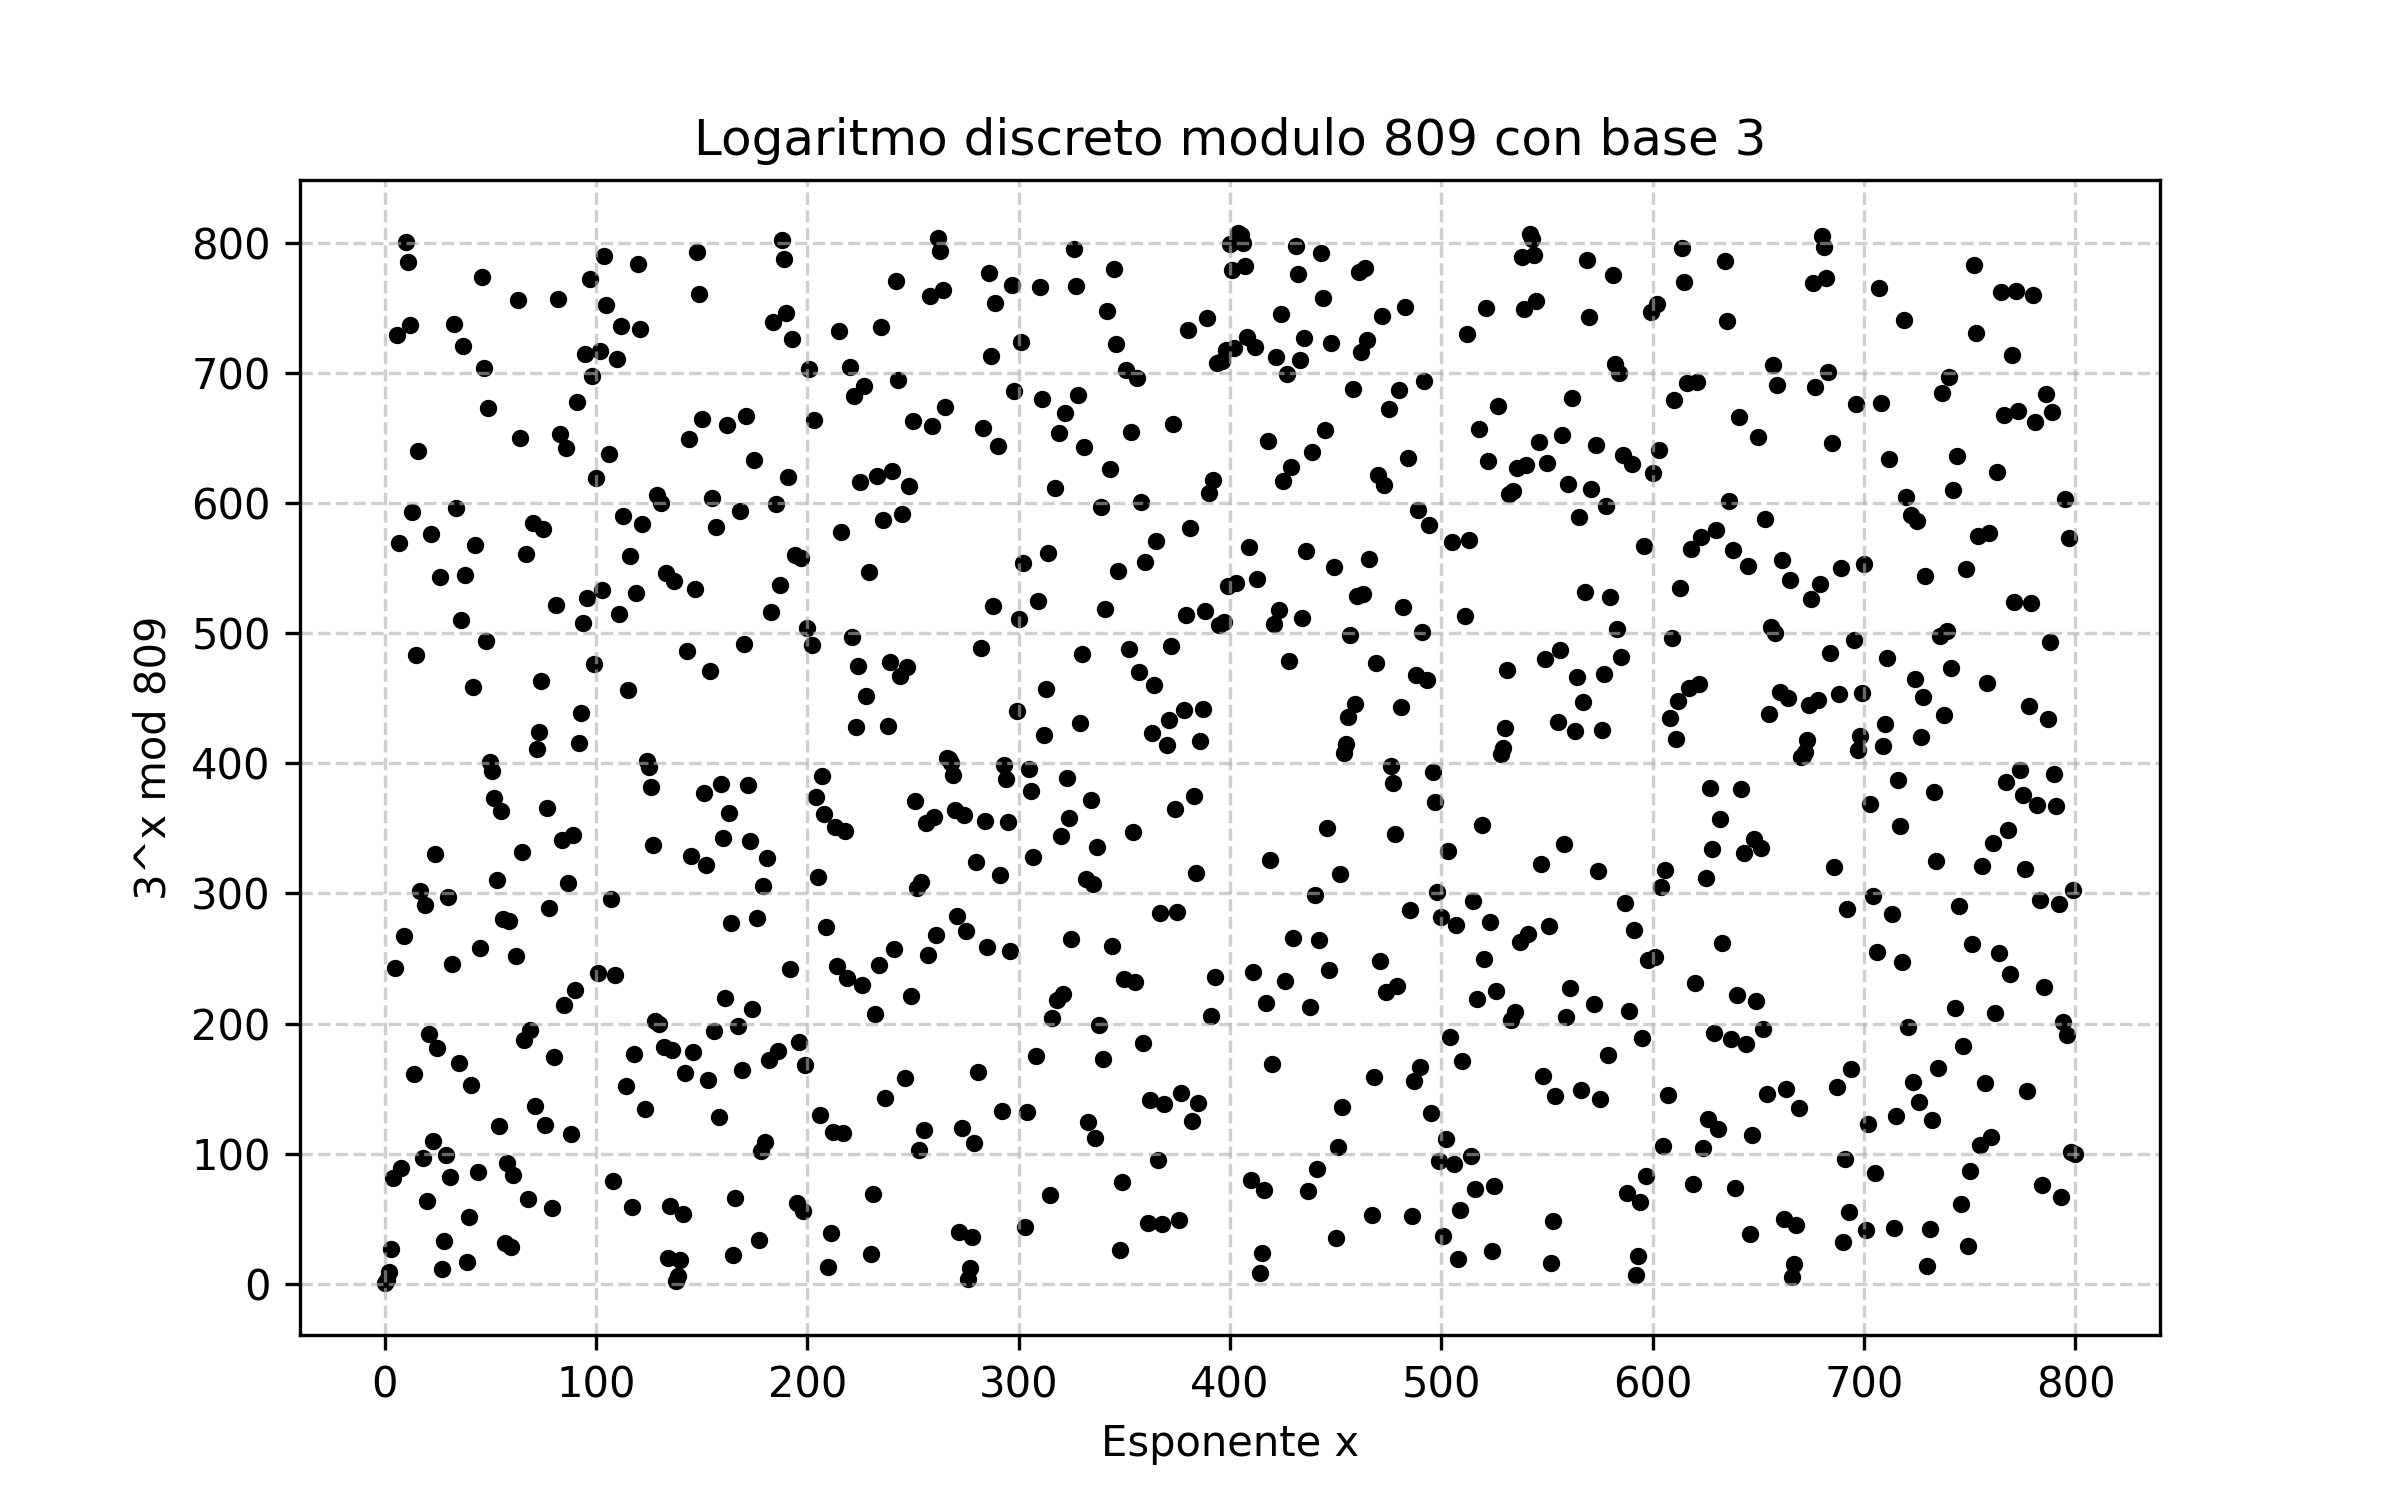
\includegraphics[width=\textwidth]{images/logaritmo_discreto.png}
    \caption{Grafico del logaritmo discreto.}
    \label{fig:discreto}
  \end{subfigure}
  \hfill
  \begin{subfigure}{0.48\textwidth}
    \centering
    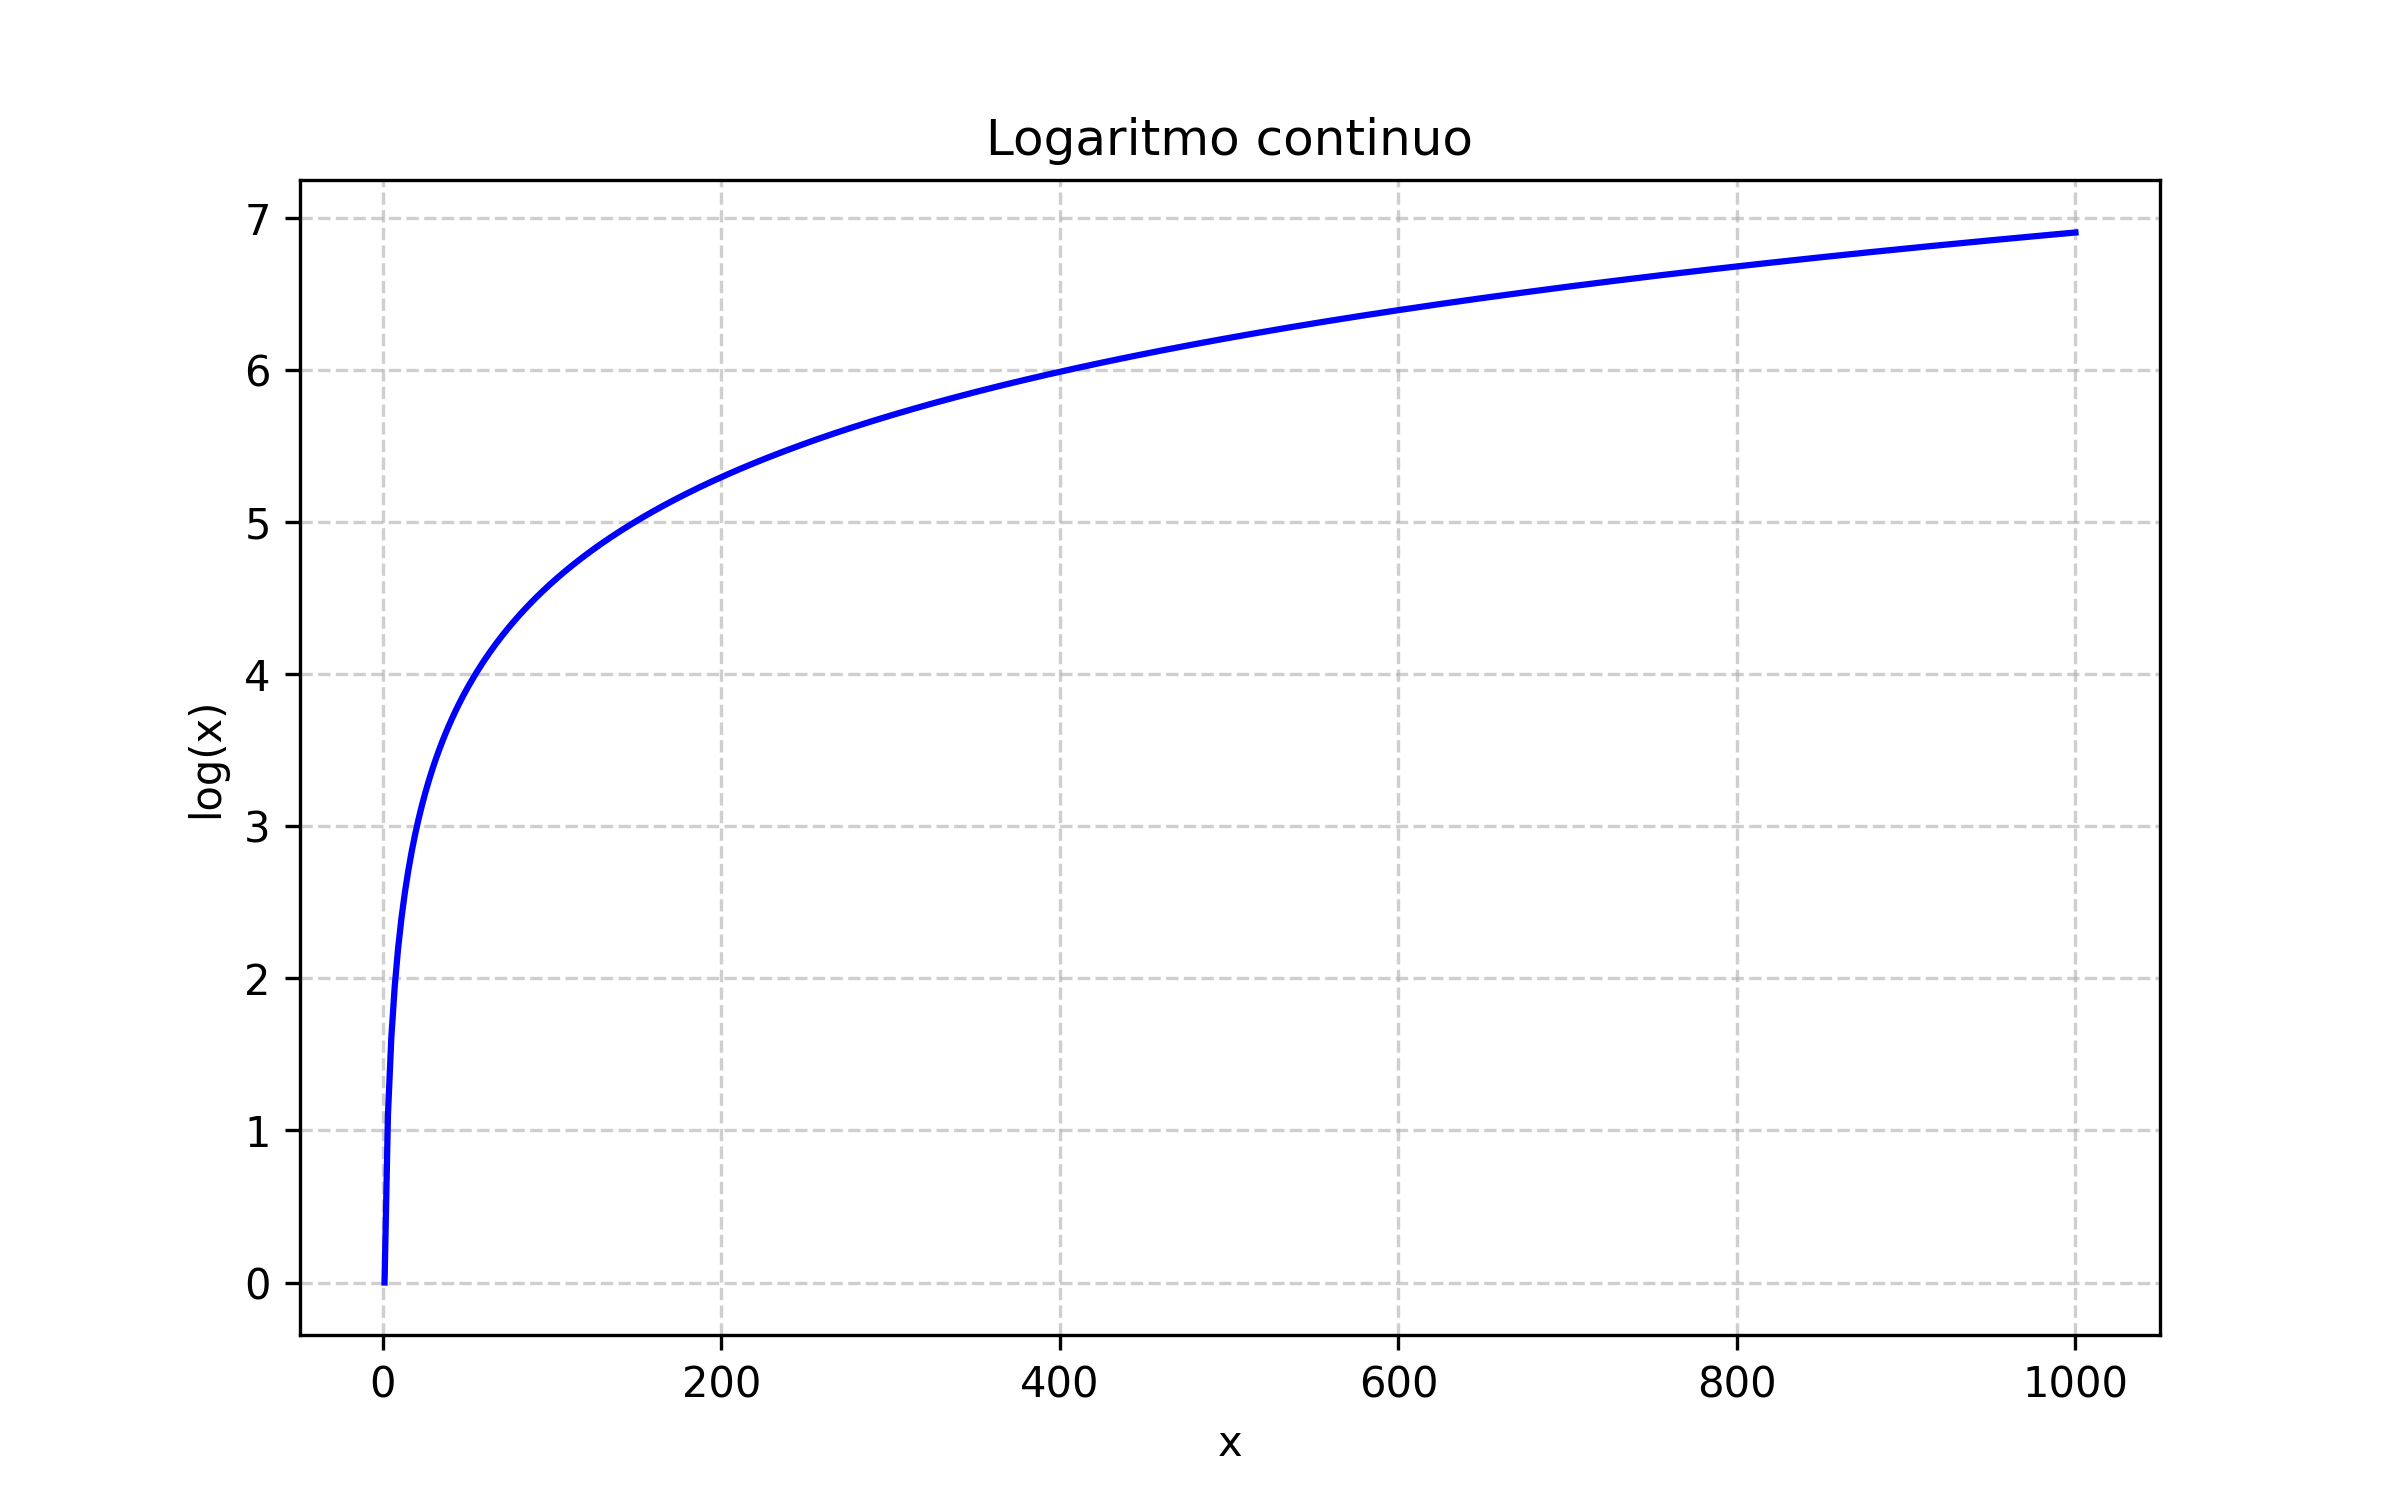
\includegraphics[width=\textwidth]{images/logaritmo_continuo.png}
    \caption{Grafico del logaritmo continuo.}
    \label{fig:continuo}
  \end{subfigure}
  \caption{Confronto tra logaritmo discreto e logaritmo continuo.}
  \label{fig:logaritmi}
\end{figure}

Il motivo principale per cui il logaritmo discreto risulta difficilmente calcolabile, a differenza del logaritmo continuo, risiede nella struttura discreta e ciclica del gruppo modulare.
Come mostrato in \autoref{fig:discreto}, i punti ottenuti mediante l'esponenziazione modulare risultano distribuiti in maniera apparentemente casuale all'interno del piano cartesiano, senza seguire un andamento regolare o monotono.
La funzione esponenziale modulo $p$, infatti, non è monotona e presenta un comportamento periodico, il che rende impossibile definire un'inversa diretta e, di conseguenza, calcolare agevolmente il logaritmo discreto.

\section{AES-GCM}\label{sec:aes}

L'\textbf{AES (Advanced Encryption Standard)}, conosciuto anche come \textbf{Rijndael}, sviluppato da J. Daemen and V. Rijmen, il cui funzionamento è descritto nel libro \textit{The Design of Rijndael: AES - The Advanced Encryption Standard} \cite{book}, è un algoritmo di cifratura simmetrica a blocchi, standardizzato dal NIST (National Institute of Standards and Technology) nel 2001 per sostituire il precedente DES (Data Encryption Standard). È oggi uno degli algoritmi crittografici più utilizzati al mondo, grazie alla sua sicurezza e all’efficienza sia su hardware che su software

Rijndael è una rete a sostituzione e permutazione. È veloce sia se sviluppato in software sia se sviluppato in hardware, è relativamente semplice da implementare, richiede poca memoria e offre un buon livello di protezione, motivi che complessivamente l'hanno reso il preferito rispetto agli altri algoritmi proposti. Nell'AES il blocco è di dimensione fissa (128 bit) e la chiave può essere di 128, 192 o 256 bit.

L’\textbf{AES-GCM (Galois/Counter Mode)}, descritto nello standard RFC 5288 \textit{AES Galois Counter Mode
(GCM) Cipher Suites for TLS} \cite{rfc5288}, è una modalità di utilizzo di AES che fornisce cifratura autenticata.
Questo significa che garantisce sia confidenzialità, ossia i dati sono cifrati con AES in modalità CTR (Counter Mode), oltre a garantire integrità e autenticità, ovvero un tag di autenticazione assicura che i dati non siano stati alterati.
AES-GCM è oggi una delle modalità più diffuse, usata in protocolli come SSH, QUIC/HTTP3, e nel Wi-Fi moderno.

\section{SHA-256}\label{sec:sha}

Una \textbf{funzione di hash crittografica (CHF)} è un algoritmo che associa un input arbitrario a un output di lunghezza fissa $n$ bit, garantendo proprietà fondamentali per la sicurezza:

\begin{itemize}
    \item \textbf{Uniformità}: ogni valore di hash ha probabilità $2^{-n}$ di comparire.
    \item \textbf{Resistenza alla preimmagine}: dato un hash, è computazionalmente infattibile ricavare l'input corrispondente ($\approx 2^n$ tentativi).
    \item \textbf{Resistenza alla seconda preimmagine}: data una stringa, è difficile trovarne un'altra con lo stesso hash.
    \item \textbf{Resistenza alle collisioni}: è improbabile trovare due input distinti con lo stesso hash; la complessità attesa è $2^{n/2}$.
\end{itemize}

\texttt{SHA-256} (Secure Hash Algorithm 256-bit) \cite{FIPS180-4} è una funzione di hash crittografica appartenente alla famiglia \texttt{SHA-2}, progettata dalla National Security Agency (NSA) e pubblicata dal NIST nel 2001 come successore di \texttt{SHA-1}.

\texttt{SHA-256} produce un digest di 256 bit, ossia una stringa di 64 caratteri esadecimali, indipendentemente dalla dimensione del messaggio in ingresso. Questa proprietà consente di trattare l'hash come una sorta di "impronta digitale" univoca del dato, utile per verificarne l'integrità e l'autenticità senza dover conservare l'intero contenuto originale.

Dal punto di vista operativo, l'algoritmo segue una struttura tipica delle funzioni di hash della famiglia Merkle–Damgård: al messaggio viene aggiunto inizialmente del padding e suddiviso in blocchi di 512 bit, che vengono elaborati iterativamente da una funzione di compressione basata su operazioni bitwise, somme modulari e funzioni non lineari. Alla fine di questa elaborazione, lo stato interno dell'algoritmo viene trasformato nell'hash finale di 256 bit.

Grazie a questa costruzione, \texttt{SHA-256} è oggi uno degli algoritmi più utilizzati in ambito crittografico. Viene impiegato in protocolli come TLS e IPsec, nei sistemi di firma digitale come DSA ed ECDSA, oltre ad avere un ruolo cruciale nel funzionamento delle blockchain e dei sistemi di proof-of-work, dove garantisce l'imprevedibilità e la verificabilità delle operazioni.